\chapter{Finite Element Method Details}
\label{app:FEMIntegrals}
The definitions of the basis functions of the finite element method used by $\text{FEVM}_2$ described in Chapter \ref{chp:HFVMMethod} and the function spaces mentioned in Chapter \ref{chp:HFVMMethod} are provided here. Beginning with the basis function definitions.

\section{Basis Functions}
Since all integrals of the basis functions are calculated with respect to the variable $\xi$, the basis functions are given in terms of $\xi$. The mapping from the $x$-space of the numerical grid to the canonical $\xi$-space is
\begin{equation*}
x = x_j + \xi \frac{\Delta x}{2}.
\end{equation*}
This mapping takes the $j^{th}$ cell $\left[x_{j-1/2},x_{j+1/2}\right]$ in the $x$-space to the interval $\left[-1,1\right]$ in the $\xi$-space.

The basis functions $\psi$ for $h$ and $G$ shown in Figure \ref{fig:P1DiscBasisAPP} are
\begin{subequations}
	\label{eqn:App1:PsiDef}
\begin{align}
\psi^+_{j-1/2} &= \left\lbrace \begin{array}{c c}
\frac{1}{2}\left(1 - \xi\right) & -1 \le \xi \le 1\\
0 & \text{otherwise} ,
\end{array} \right.  \\
\psi^-_{j+1/2} &= \left\lbrace \begin{array}{c c}
\frac{1}{2}\left(1 + \xi\right) & -1 \le \xi \le 1\\
0 & \text{otherwise} .
\end{array} \right. 
\end{align}
\end{subequations}

\begin{figure}
	\centering
	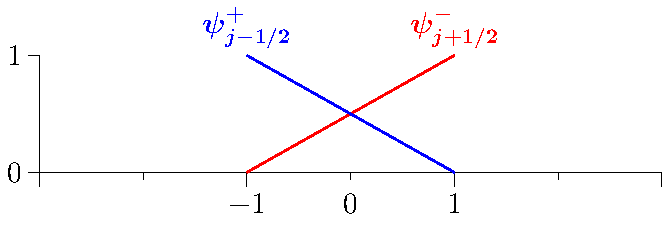
\includegraphics[width=0.8\textwidth]{./app1/Figures/P1.pdf}
	\caption{Support of the discontinuous linear basis functions $\psi$ in the $\xi$-space.}
	\label{fig:P1DiscBasisAPP}
\end{figure}

The basis functions $\phi$ for $u$ and the test function $v$ displayed in Figure \ref{fig:P2ContBasisAPP} are given by
\begin{subequations}
	\label{eqn:App1:PhiDef}
\begin{align}
\phi_{j-1/2} &= \left\lbrace \begin{array}{c c}
2 \left(\xi + \frac{3}{2}\right)\left(\xi + 2\right) & -2 \le \xi \le -1\\
\frac{1}{2}\xi(\xi - 1) & -1 \le \xi \le 1\\
0 & \text{otherwise} ,\end{array} \right.  \\
\phi_{j} &= \left\lbrace \begin{array}{c c}
-\left(\xi - 1\right)\left(\xi + 1\right) & -1 \le \xi \le 1\\
0 & \text{otherwise},
\end{array} \right.  \\ 
\phi_{j+1/2} &= \left\lbrace \begin{array}{c c}
\frac{1}{2}\xi(\xi + 1) & -1 \le \xi \le 1\\
2\left(\xi - 2\right)\left(\xi - \frac{3}{2} \right) & 1 \le \xi \le 2\\
0 & \text{otherwise}.
\end{array} \right. 
\end{align}
\end{subequations}
\begin{figure}
	\centering
	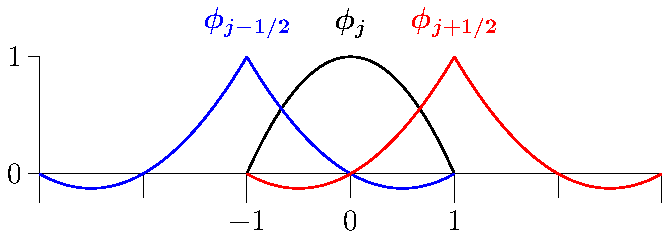
\includegraphics[width=0.8\textwidth]{./app1/Figures/P2.pdf}
	\caption{Support of the continuous piecewise quadratic basis functions $\phi$ in the $\xi$-space.}
	\label{fig:P2ContBasisAPP}
\end{figure}

Finally the basis functions $\gamma$ for the bed profile $b$ displayed in Figure \ref{fig:P3ContBasis} are given by
\begin{subequations}
	\label{eqn:App1:GamDef}
\begin{align}
\gamma_{j-1/2} &= \left\lbrace \begin{array}{c c}
\frac{9}{2}\left(\xi + \frac{4}{3}\right)\left(\xi + \frac{5}{3}\right)\left(\xi + 2\right) & -2 \le \xi \le -1\\
\frac{9}{16}\left(\xi - 1\right)\left(\xi - \frac{1}{3}\right)\left(\xi  + \frac{1}{3}\right) & -1 \le \xi \le 1\\
0 & \text{otherwise}, 
\end{array} \right. \\
\gamma_{j-1/6} &= \left\lbrace \begin{array}{c c}
\frac{27}{16}\left(\xi - 1\right)\left(\xi - \frac{1}{3}\right)\left(\xi + 1\right) & -1 \le \xi \le 1\\
0 & \text{otherwise}, 
\end{array} \right. \\
\gamma_{j+1/6} &= \left\lbrace \begin{array}{c c}
-\frac{27}{16}\left(\xi - 1\right)\left(\xi + \frac{1}{3}\right)\left(\xi + 1\right) & -1 \le \xi \le 1\\
0 & \text{otherwise} ,
\end{array} \right. \\
\gamma_{j-1/2} &= \left\lbrace \begin{array}{c c}
\frac{9}{16}\left(\xi + 1\right)\left(\xi - \frac{1}{3}\right)\left(\xi  + \frac{1}{3}\right) & -1 \le \xi \le 1\\
-\frac{9}{2}\left(\xi - \frac{4}{3}\right)\left(\xi - \frac{5}{3}\right)\left(\xi - 2\right) & 1 \le \xi \le 2\\
0 & \text{otherwise} .
\end{array} \right. 
\end{align}
\end{subequations}

\begin{figure}
	\centering
	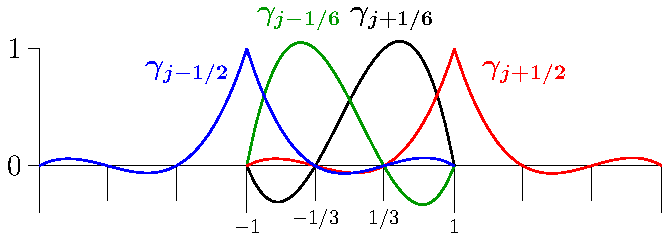
\includegraphics[width=0.8\textwidth]{./app1/Figures/P3.pdf}
	\caption{Support of the continuous piecewise cubic basis functions $\gamma$ in the $\xi$-space.}
	\label{fig:P3ContBasisAPP}
\end{figure}

The calculation of the derivatives of these basis functions with respect to $\xi$ are straightforward and hence omitted. 

\section{Function Spaces}
The function spaces mentioned in Chapter \ref{chp:HFVMMethod} are the space of square integrable functions $\mathbb{L}^2(\Omega)$ and the Sobolev space $\mathbb{W}^{k,2}(\Omega)$. To be precise we now define these function spaces here. 

A function $f(x)$ is in $\mathbb{L}^2(\Omega)$ if
\begin{equation*}
\left( \int_{\Omega} f(x)^2 \; dx \right)^{\frac{1}{2}} < \infty.
\end{equation*}

While $f(x)$ is in $\mathbb{W}^{k,2}(\Omega)$ if 
\begin{equation*}
\left( \int_{\Omega} f(x)^2 \; dx + \sum^k_{j=1}  \int_{\Omega} \left[D^j f(x) \right]^2 \; dx  \right)^{\frac{1}{2}} < \infty.
\end{equation*}
where $D^j f(x)$ is the $j^{th}$ weak derivative of $f(x)$. 
